
\subsection{PX4 Integration via MAVROS}
MAVROS serves as the communication bridge between ROS 2 and the Pixhawk 6X Pro flight controller \cite{mavros_wiki}. It receives the corrected ENU pose from the VIO Bridge on \texttt{/mavros/vision\_pose/pose} and automatically converts it to the NED convention before packing it into a \texttt{VISION\_POSITION\_ESTIMATE} MAVLink message and sending it to the flight controller via the Holybro Jetson Pack's integrated UART connection \cite{holybro_jetson_pack,px4_user_guide}.\par

\begin{figure}[!ht]
    \centering
    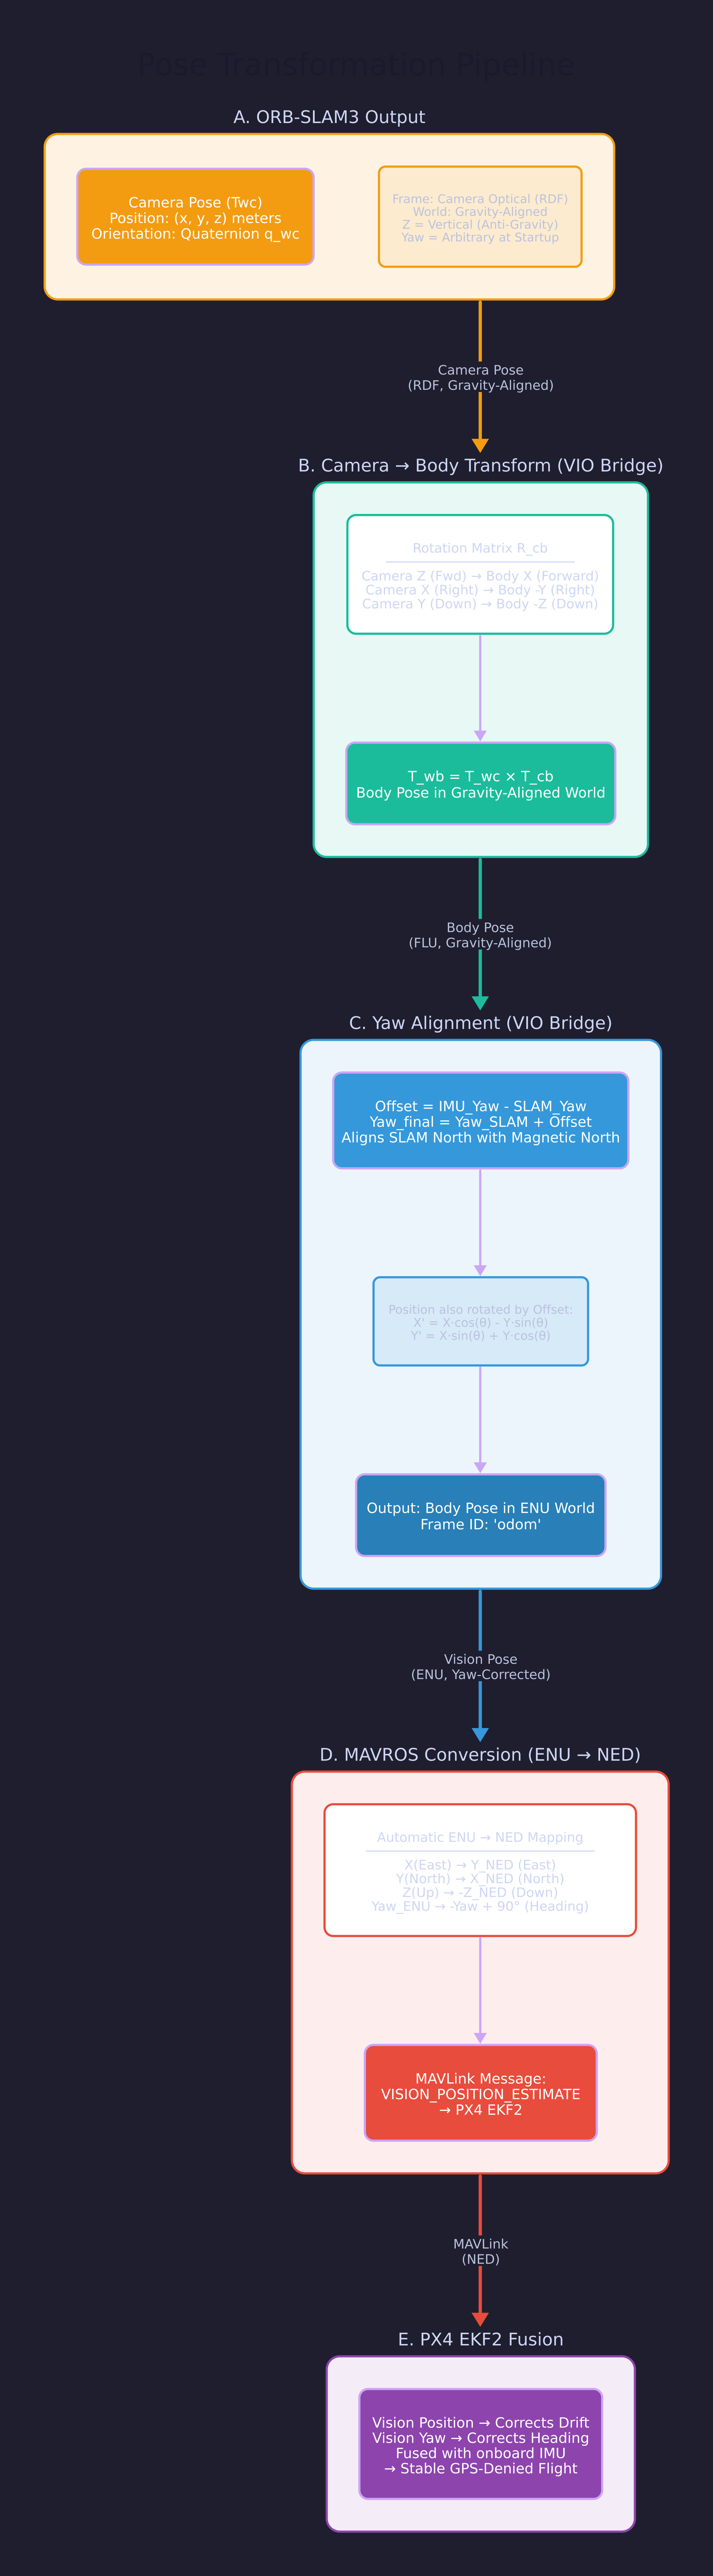
\includegraphics[width=\linewidth,height=0.75\textheight,keepaspectratio]{images/03_pose_pipeline.jpg}
    \caption{Pose Transformation Pipeline}
    \label{fig:pose_transformation}
\end{figure}

\noindent\textbf{ENU $\rightarrow$ NED Conversion (MAVROS):} MAVROS converts the incoming ENU vision pose into the PX4-friendly NED convention as follows:
\begin{itemize}
    \item $X_{\text{NED}} = Y_{\text{ENU}}$ (North)
    \item $Y_{\text{NED}} = X_{\text{ENU}}$ (East)
    \item $Z_{\text{NED}} = -Z_{\text{ENU}}$ (Down)
    \item $\textit{Yaw}_{\text{NED}} = -\textit{Yaw}_{\text{ENU}} + 90^\circ$
\end{itemize}

\begin{table}[H]
\centering
\scriptsize % reduces font size
\caption{PX4 EKF2 Parameters for Vision Fusion}
\resizebox{\textwidth}{!}{%
\begin{tabular}{|p{3.6cm}|p{2.2cm}|p{9.8cm}|}
\hline \textbf{Parameter} & \textbf{Value} & \textbf{Description} \\
\hline EKF2\_EV\_CTRL & 15 & Enable Vision Position, Yaw, Velocity, and Height fusion \\
\hline EKF2\_HGT\_REF & 3 & Set height reference to Vision \\
\hline EKF2\_GPS\_CTRL & 0 & Disable GPS fusion (indoor operation) \\
\hline EKF2\_EV\_DELAY & 50\,ms & Vision processing latency compensation \\
\hline EKF2\_EVP\_NOISE & 0.1 & Vision position noise (confidence) \\
\hline EKF2\_EVA\_NOISE & 0.1 & Vision angle noise (confidence) \\
\hline EKF2\_EV\_POS\_X/Y/Z & 0.0 & Camera-to-IMU offset (measure physically) \\
\hline
\end{tabular}}
\label{tab:px4_ekf2_params_vision}
\end{table}

\subsection{Coordinate Systems and Transformations}
Correct coordinate frame handling is the single most critical aspect of the VIO integration. The system uses four distinct coordinate frames, each with a specific convention. The transformation pipeline flows as: Camera Optical (RDF) $\rightarrow$ [${R}_{cb}$ rotation] $\rightarrow$ Body (FLU) $\rightarrow$ [Yaw correction] $\rightarrow$ World (ENU) $\rightarrow$ [MAVROS auto-conversion] $\rightarrow$ PX4 (NED) $\rightarrow$ [EKF2 fusion] $\rightarrow$ Stable Flight.

\begin{figure}[!ht]
    \centering
    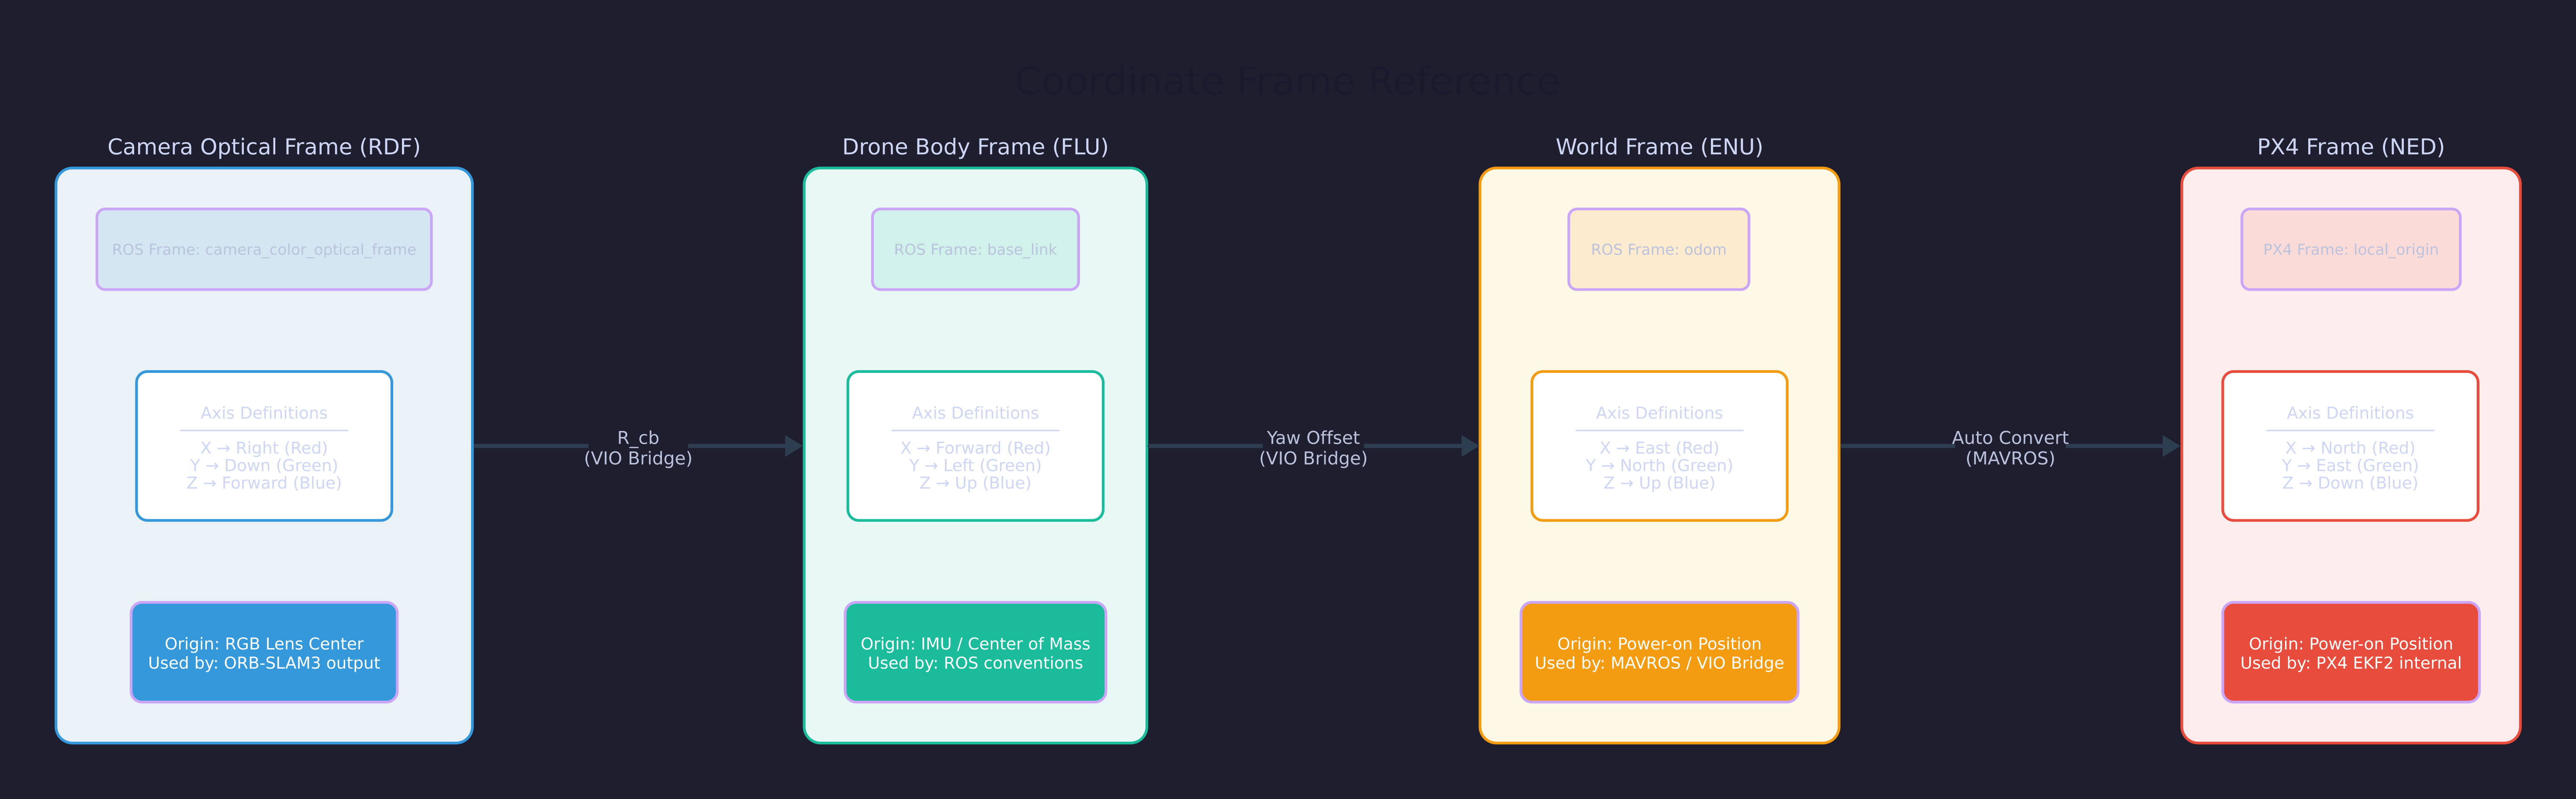
\includegraphics[width=\linewidth,height=0.75\textheight,keepaspectratio]{images/04_coordinate_frames.jpg}
    \caption{Coordinate Frames}
    \label{fig:coordinate_frames}
\end{figure}

\begin{table}[H]
\centering
\scriptsize % reduces font size
\caption{Coordinate Frames Used in the VIO Pipeline}
\resizebox{\textwidth}{!}{%
\begin{tabular}{|p{2.8cm}|p{1.6cm}|p{2.6cm}|p{1.7cm}|p{1.7cm}|p{1.7cm}|p{3.4cm}|}
\hline \textbf{Frame} & \textbf{Convention} & \textbf{ROS Frame ID} & \textbf{X Axis} & \textbf{Y Axis} & \textbf{Z Axis} & \textbf{Used By} \\
\hline Camera Optical & RDF & \texttt{camera\_link} & Right & Down & Forward & ORB-SLAM3 \\
\hline Drone Body & FLU & \texttt{base\_link} & Forward & Left & Up & ROS~2 / VIO Bridge \\
\hline World & ENU & \texttt{odom} & East & North & Up & MAVROS \\
\hline PX4 Internal & NED & \texttt{local\_origin} & North & East & Down & Pixhawk~6X Pro \\
\hline
\end{tabular}}
\label{tab:coordinate_frames}
\end{table}

\subsection{Sensor Calibration}
Accurate calibration is essential for SLAM performance. The following calibration procedures were performed:

\begin{table}[H]
\centering
\scriptsize % reduces font size
\caption{Sensor Calibration Procedures}
\resizebox{\textwidth}{!}{%
\begin{tabular}{|p{3.0cm}|p{6.5cm}|p{7.0cm}|}
\hline \textbf{Procedure} & \textbf{Method} & \textbf{Purpose} \\
\hline Camera Intrinsics & Extracted from \texttt{/camera/color/camera\_info} topic (factory calibration from Orbbec SDK). Verified with checkerboard pattern. & Provides focal lengths (fx=606.96, fy=607.11), principal point (cx=637.73, cy=392.85), and distortion coefficients for accurate feature localization. \\
\hline IMU-Camera Extrinsics & Derived from the static TF between \texttt{camera\_gyro\_optical\_frame} and \texttt{camera\_color\_optical\_frame}. Translation offset of 25\,mm along X-axis. & Defines the rigid 6-DOF transformation ($T_{bc}$) between the IMU and the camera, allowing ORB-SLAM3 to correctly fuse inertial and visual data. \\
\hline IMU Noise Parameters & Empirically tuned --- gyroscope noise: $2.0 \times 10^{-2}$\,rad/s/$\sqrt{\text{Hz}}$, accelerometer noise: $2.0 \times 10^{-1}$\,m/s$^{2}$/$\sqrt{\text{Hz}}$. Values set higher than datasheet specifications. & Deliberately inflated noise values improve initialization stability and prevent the optimizer from trusting noisy consumer-grade IMU data too heavily. \\
\hline
\end{tabular}}
\label{tab:sensor_calibration_procedures}
\end{table}


\subsection{Unified Launch System}
A unified ROS 2 launch file (\texttt{vio\_system.launch.py}) orchestrates the startup of all four nodes with staggered timing to ensure proper initialization order and data availability:
\begin{figure}[!ht]
    \centering
    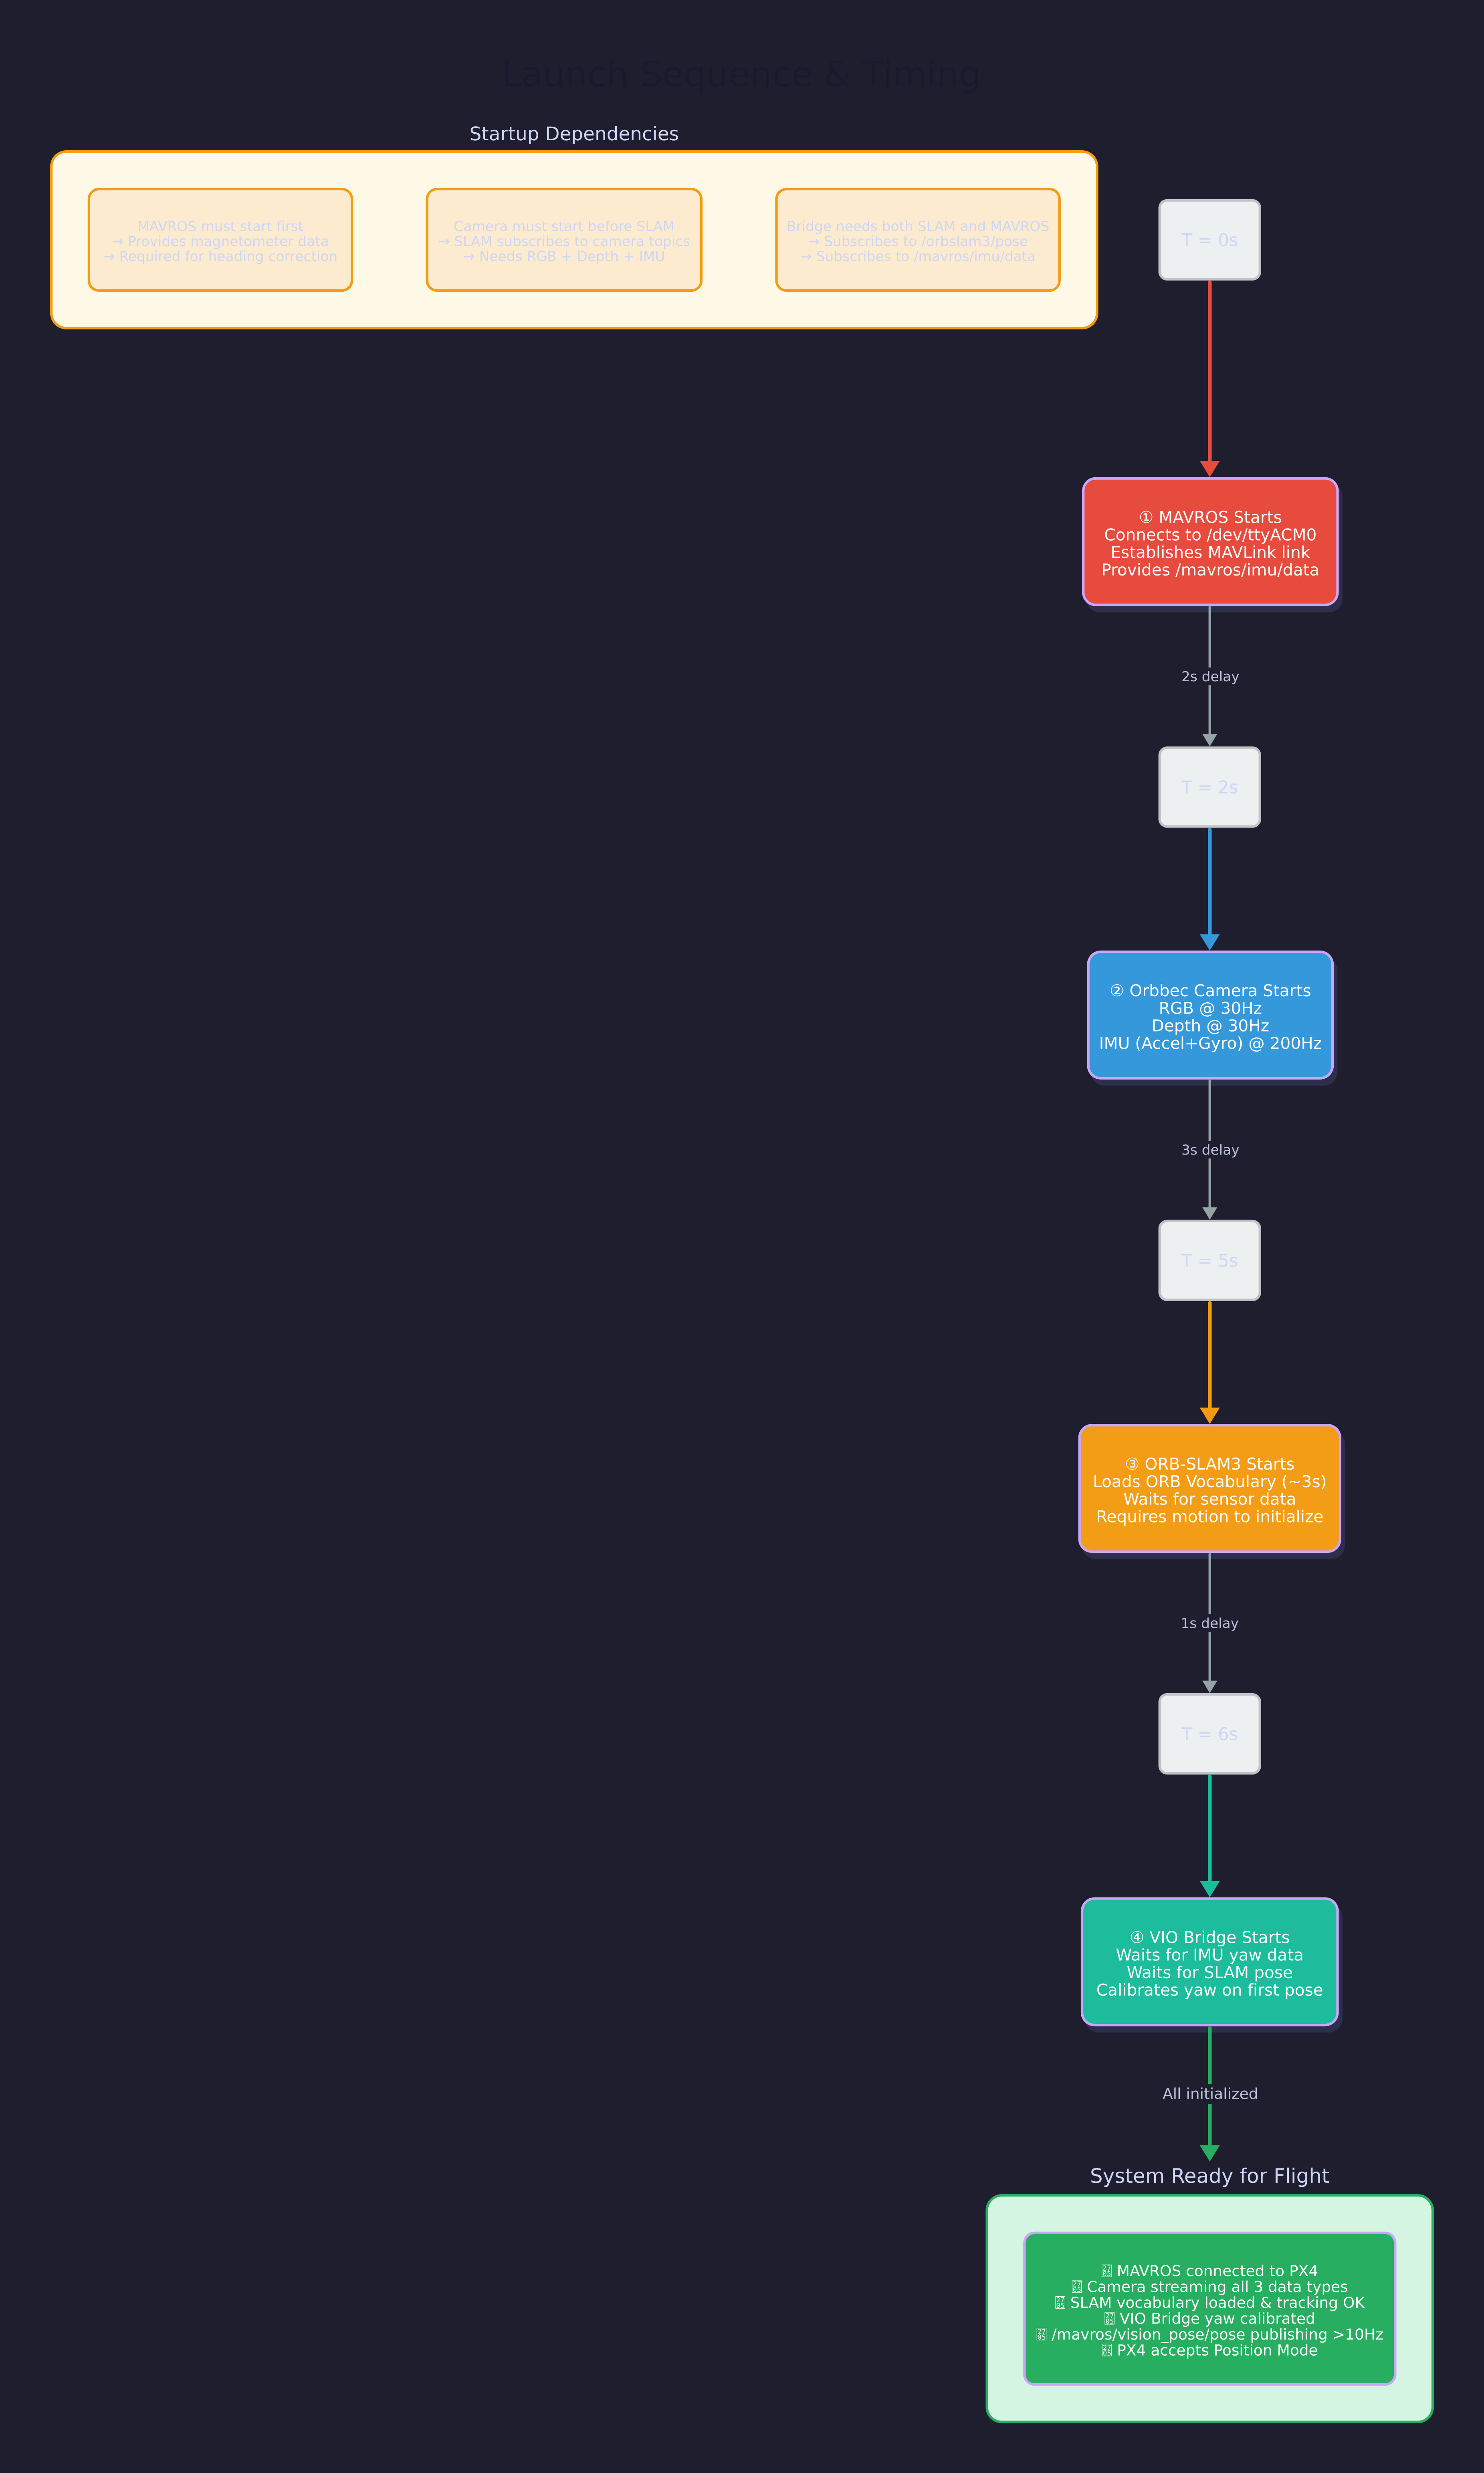
\includegraphics[width=\linewidth,height=0.75\textheight,keepaspectratio]{images/07_launch_sequence.jpg}
    \caption{Launch Sequence}
    \label{fig:launch_sequence}
\end{figure}
\begin{table}[H]
\centering
\scriptsize % reduces font size
\caption{Staggered Launch Schedule for VIO System Nodes}
\resizebox{\textwidth}{!}{%
\begin{tabular}{|p{2.0cm}|p{3.0cm}|p{9.2cm}|p{4.0cm}|}
\hline \textbf{Delay} & \textbf{Node} & \textbf{Reason} & \textbf{Ready Signal} \\
\hline T = 0\,s & MAVROS & Starts first --- must provide magnetometer data to VIO Bridge for heading correction & FCU connection established \\
\hline T = 2\,s & Orbbec Camera & Camera topics must be available before ORB-SLAM3 subscribes & Image and IMU topics publishing \\
\hline T = 5\,s & ORB-SLAM3 & Needs $\sim$3\,s to load vocabulary file (\texttt{ORBvoc.txt}); requires camera data already flowing & ``Vocabulary loaded'' log message \\
\hline T = 6\,s & VIO Bridge & Needs both SLAM pose and MAVROS IMU to be active & \texttt{/mavros/vision\_pose/pose} publishing $>10$\,Hz \\
\hline
\end{tabular}}
\label{tab:launch_schedule}
\end{table}

The launch file exposes configurable arguments for vocabulary path, ORB-SLAM3 config file, FCU URL, GCS URL, and toggles for the SLAM visualizer and magnetometer correction.